\chapter{Liquids, Gases, and Phase Transitions}
\label{chapter:liquids_and_gases}

%\section*{Objectives}
%
%\begin{objectives}
%\item Describe qualitatively why melting and vaporization phase
%  transitions occur, and what their associated latent heats are.
%  Apply latent heats quantitatively to heat flow problems.
%
%\item Relate thermal kinetic energy, thermal speed, and temperature for
%a solid, liquid, or gas.
%
%\item Describe the properties of monatomic and diatomic ideal gases, including
%their molar specific heat and speed of sound.
%
%\item Relate pressure to forces acting on a surface, and be able to
%qualitatively explain pressure by considering the motion of gas molecules.
%
%\item Relate pressure, volume, temperature, and number of molecules or
%moles, or changes in the quantities, using the ideal gas law.
%
%\end{objectives}


In this chapter we study the liquid and gas states of matter, as
well as the phase transitions that occur when going from solid to
liquid or from liquid gas.  As before with the solid state, our tools
for understanding these states will be the molecular pair potential
and the equipartition theorem.

\section{Phases of Matter}

%[General words about the liquid and gas states of matter, in contrast
%to the solid state.]

Since the dawn of human existence, people have noticed that
matter could be solid, liquid, or gas.  What cavewoman Thag and her
contemporaries did not realize is that these quite different phases
are made up of the same stuff: molecules that are 
pushing and pulling on each other, sometimes in a solid phase, sometimes
a liquid and sometimes a gas.  
She was not the only one who didn't understand this.  Plato didn't
know about molecules.  Nor did Dante, or even Newton.  Only after the
seminal work of Boltzmann and Einstein around the turn of the 20$^{\rm th}$ 
century did our process of scientific discovery lead us to understand the
molecular form of matter.  

This discovery is one of the crowning achievements of our species, and
is also very practical, having provided the basis for most of our
modern technology.  The great 20th century physicist Richard
Feynman\footnote{You're going to be hearing more about him in PHYS
  212.} once remarked
\begin{quote}
  ``If, in some cataclysm, all scientific knowledge were to be
  destroyed, and only one sentence passed on to the next generation of
  creatures, what statement would contain the most information in the
  fewest words? I believe it is the atomic hypothesis \dots that all
  things are made of atoms --- little particles that move around in
  perpetual motion, attracting each other when they are a little
  distance apart, but repelling upon being squeezed into one
  another. In that one sentence you will see an enormous amount of
  information about the world, if just a little imagination and
  thinking are applied.''
\end{quote}
Let us now follow Feynman's suggestion and apply a little
imagination and thinking.

We have been discussing the solid phase of matter, where the particles
are arranged in a regular lattice pattern, and the forces between the
particles can be well-modeled as springs attached between neighbors.
But we know from everyday experience that a solid can be melted when
heated enough.  Consider a lattice of vibrating molecules.  Once the
molecular excursions become large enough, the molecules start slipping
past one another.  As a result, the regular arrangement of the
molecules in the lattice breaks down and the molecules are now
disordered.  They are still very closely packed and the density is
comparable to the solid state, but the object has no rigidity.  This
is a liquid.


\begin{figure}
\begin{center}
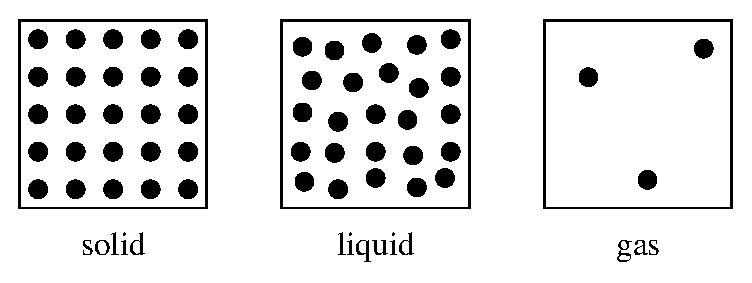
\includegraphics[width=3.5in]{liquids_and_gases/phases.eps}
\caption{The molecular picture of the phases of matter.}
\label{fig:phases}
\end{center}
\end{figure}


For most substances, there exists a boiling point separating a liquid
phase from a gas phase.  The picture you should have for the gas state
is molecules moving about freely, far from their neighbors, and moving
in a straight line until they collide with another molecule or with
the walls of the container.  Like a liquid, the gas phase is
disordered.  But the density of gases is much lower than liquids.
Another difference between liquids and gases that we can understand
immediately from the molecular viewpoint is their compressibility.
Because the gas is dilute, we can compress a gas if we push the walls
of the container inward. The molecules end up a bit closer together
and bounce around a little faster, but otherwise they don't object.
Liquids are essentially incompressible: you can't squeeze water to fit
into a smaller volume.  The liquid molecules are already packed
together, albeit in a messy way, and any further squeezing is resisted
by the repulsive forces of the pair potential.

Our basic understanding of the thermal energy of matter, developed
in sections \ref{section:thermal_kinetic_energy} and
\ref{section:thermal_potential_energy} for solids 
applies for liquids and gases as well: in particular, 
thermal kinetic energy is associated with motion of the molecules.
And the potential energy associated with
the forces between the molecules --- i.e., the pair potential ---
provides the thermal potential energy.
However, there are significant differences in the thermal
potential energy for the different phases:
\begin{itemize}
\item in the solid phase are the molecules very near their equilibrium
  separation, allowing us to approximate their forces with springs
\item in the liquid phase, however, the potential energy is
  complicated, since the molecules are pushed closer together and
  pulled farther apart as the molecules squeeze by each other, making
  the spring approximation invalid, and
\item in the gas phase, the molecules are so far apart that, except for
  very brief collisions, there is no potential energy.
\end{itemize}

In contrast to these differences, the thermal {\it kinetic energy\/}
is identical in form in all three phases.  This allows us to develop the
notion of thermal speed.

\section{Thermal Speed}

%[General use of equipartition to learn about the kinetic energy and
%  therefore the speed of the molecules, regardless of phase.  Mention
%  the displacement from eq in a solid, also.]
For all phases of matter,  the translational kinetic
energy of a single molecule is
\begin{equation}
K_\text{trans} = {\textstyle\frac{1}{2}} m v_x^2 + 
{\textstyle\frac{1}{2}} m v_y^2 + {\textstyle\frac{1}{2}} m v_z^2.
\label{eq:k_molecule}
\end{equation}
We can take advantage of this to determine how fast the molecules are
moving at some given temperature $T$.
Via the equipartition theorem, we can say that the average
translational kinetic energy is
\begin{equation}
\langle K_\text{trans}\bigr\rangle = \textstyle
  \bigl\langle\frac{1}{2}mv_x^2\bigr\rangle 
  +\bigl\langle\frac{1}{2}mv_y^2\bigr\rangle 
  +\bigl\langle\frac{1}{2}mv_z^2\bigr\rangle 
= \frac{3}{2}k_BT,   \quad\text{(single molecule)}
\end{equation}
since there are three quadratic terms in the energy.  Recalling that
$v^2=v_x^2+v_y^2+v_z^2$, we can write
\begin{equation}
%\langle K_\text{trans}\rangle = 
  \frac{3}{2}k_BT = \textstyle\bigl\langle \frac{1}{2}mv^2\bigr\rangle = 
  \frac{1}{2}m\langle v^2\rangle \quad\Rightarrow\quad
  \langle v^2\rangle = 3 k_B T/m.
\end{equation}
Now we define the thermal speed, which indicates the typical speed of
the molecules, as\footnote{Why didn't we simply define
  $v_\text{therm}$ as the average velocity $\langle \vec v\rangle$?
  Because the average velocity is zero, which tells us nothing about
  the typical magnitude of the velocity.}
\begin{equation}
  v_\text{therm} =  \sqrt{\langle v^2\rangle}= \sqrt{\frac{3k_BT}{m}} = 
  \sqrt{\frac{3RT}{M}}
\label{eq:v_thermal}
\end{equation}
where $m$ is the molecular mass and $M$ is the molar
mass.\footnote{A.k.a. what is often horribly called the ``molecular
  weight'' (horrible because its a mass, not a weight, and it's for a
  mole of molecules, not just one).  From here on, we'll abandon that
  nonsensical term and call it molar mass.} The second equality above
comes from multiplying numerator and denominator by $N_A$ and then
using $M = N_A m$ and $R=N_Ak_B$.  So we have shown, via
equipartition, a direct connection between the temperature and the
translational kinetic energy.

% Here again we have used the idea
%that temperature is related to translational kinetic energy of the
%molecules.\footnote{Again, a more general definition of temperature
%  will be provided in Chapter \ref{chapter:second_law}.}  And now we
%can say that temperature related to the speed of the molecules,
%according to Eq.~(\ref{eq:v_thermal}).

\begin{example}{Speed of Nitrogen in the Atmosphere}
What is the typical speed of a nitrogen molecule in the atmosphere at 
room temperature of $22^\circ\units{C}$?
\solution
First we need to convert the temperature to Kelvin:
%\begin{equation}
$T = 273 + 22 = 295\units{K}$.
%\end{equation}
The molar mass of elemental nitrogen is $14\units{g/mol}$.  However,
nitrogen in the air is in molecular form, $N_2$, which has two nitrogen
atoms per molecule, and a molar mass of $28\units{g/mol}$.  We
may use Eq.~(\ref{eq:v_thermal}), but to be consistent with SI units,
we should convert the molar mass to kilograms:
\begin{align}
v_\text{therm} &= \sqrt{\frac{3 R T}{M}} = \sqrt{
 \frac{3(8.31\units{J/mol$\cdot$K})(295\units{K})}{0.028\units{kg/mol}}}
\nonumber\\
&= 512\units{m/s}
\end{align}
which is the same as about 1150 m.p.h.  Room temperature molecules are fast!
\label{example:vtherm}
\end{example}

A variation of this approach (i.e., using the equipartition theorem)
can be used to determine
how much a typical molecule is displaced from its
equilibrium position but in the {\em solid phase only!}  This is discussed
(along with an example) in Sec.~\ref{sec:phase_transitions}.


\section{The Liquid State}

In the liquid state, the pair potential ``springs'' are continually
pushing and pulling and then getting stretched to the distance where
they weaken and let go.  In this way, molecules freely change their
neighbors and slide past one another, which is why a liquid can flow.
In this complicated picture, it is not possible to make a simple
calculation for the thermal potential energy.  The molar specific heat
depends in a complicated way on the details of the pair potential, and
so it varies considerably from material to material.    While physicists
and chemists have developed advanced theories for describing the
liquid state, these are beyond the scope of this course.

However, if we are given a measured specific heat, such as that of
water, we can still relate changes in the thermal energy to
temperature changes via
\begin{equation}
\Delta E_\text{therm} = n C_\text{liq}\Delta T
\end{equation}
Measured values of the specific heat are given for a few different liquids
in Table~\ref{table:liquid_specific_heats}.


\begin{table}
%\hspace{0.5in}
\begin{center}
\begin{tabular}{llc}
\hline\hline
Liquid & molecule & $C$ (J/mol$\cdot$K) \\ \hline
\noalign{\smallskip}
water & H$_2$O & 75.3 \\
methanol & CH$_3$OH & 79.5 \\
ethanol & C$_2$H$_5$OH  &  112.4 \\
acetone & (CH$_3$)$_2$CO & 125.5 \\
benzene & C$_6$H$_6$ & 134.8 \\
\hline\hline
\end{tabular}
% \caption{Molar specific heats of selected liquids.  Data is taken at 
% room temperature.}

% \begin{tabular}{llc}
% \hline\hline
% Liquid & molecule & $C$ (J/mol$\cdot$K) \\ \hline
% \noalign{\smallskip}
% water & H$_2$O & 75.3 \\
% methanol & CH$_3$OH & 79.5 \\
% ethanol & C$_2$H$_5$OH  &  112.4 \\
% acetone & (CH$_3$)$_2$CO & 125.5 \\
% benzene & C$_6$H$_6$ & 134.8 \\
% \hline\hline
% \end{tabular}
 \caption{Molar specific heats of selected liquids.  Data is taken at 
 room temperature.}
\label{table:liquid_specific_heats}
\end{center}
\end{table}

Note that $C_\text{liq}$ is different than the specific heat of the 
solid state for the same material.  It is typically larger.
For example, for copper molar specific heat in the liquid phase
is $C_\text{liq} = 36.3\units{J/mol$\cdot$K}$, compared
to $C_\text{s}=24.4\units{J/mol$\cdot$K}$ in the solid phase. 


\section{The Gas State}
\label{section:TheGasState}

In the gas phase, most of the time the molecules are so far apart that
they exert no force on each other.  The exception is the brief molecular
collision, where the pair potential plays a role in determining the forces
that they exert on each other during the collision.  However, after the
collision the pair of molecules head off in their new directions with
new speeds, moving rather quickly out of range of each other and feeling
no force.  The details of the molecular collisions are complicated,
but we can avoid having to worry about them by making use of the
equipartition theorem.

The total thermal energy for a gas is, to an excellent
approximation, purely kinetic, as the molecules are too far apart to
have an appreciable potential energy.  However, the kinetic energy 
may consist of both translational and rotational kinetic energies.
For a {\it monatomic} gas molecule, such as argon, there is no
contribution to rotational kinetic energy and so
\begin{equation}
 E_\text{molecule} = K_\text{trans} = {\textstyle\frac{1}{2}} m v_x^2 + 
{\textstyle\frac{1}{2}} m v_y^2 + {\textstyle\frac{1}{2}} m v_z^2. 
\quad\text{(monatomic ideal gas)}
\label{eq:monatomic_Emolecule}
\end{equation}
There are three quadratic contributions to the energy. 
The equipartition theorem says, therefore, that the average thermal
energy per molecule is $3(\textstyle\frac{1}{2}k_BT)$.  Therefore, the
total thermal energy is
\begin{equation}
E_\text{therm} = N\langle
E_\text{molecule}\rangle =
 {\textstyle\frac{3}{2}} N k_B T = {\textstyle\frac{3}{2}} n R T.
\quad\text{(monatomic ideal gas)}
\label{eq:monatomic_ideal_gas}
\end{equation}

\begin{figure}
\begin{center}
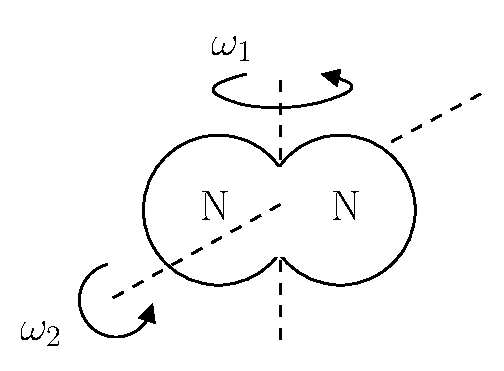
\includegraphics[width=2in]{liquids_and_gases/diatomic.eps}
\caption{Molecular nitrogen, N$_2$, has two distinct axes of rotation, 
both of which contribute to the molecular kinetic energy.}
\label{fig:diatomic}
\end{center}
\end{figure}

However, many gas molecules are diatomic, such as N$_2$, which makes up
about 78\% of our atmosphere, and O$_2$, which makes up most of the rest.
These dumbbell-shaped molecules have significant rotational kinetic energy
as well as translational kinetic energy, as shown in Fig.~\ref{fig:diatomic}.
Their molecular energy is given by
\begin{equation}
E_\text{molecule} = {\textstyle\frac{1}{2}} m v_x^2 +
{\textstyle\frac{1}{2}} m v_y^2 + {\textstyle\frac{1}{2}} m v_z^2
+{\textstyle\frac{1}{2}} I_1 \omega_1^2 + {\textstyle\frac{1}{2}} I_2
\omega_2^2
\quad\text{(diatomic ideal gas)}
\label{eq:diatomic_Emolecule}
\end{equation}
where $\omega_1$ and $\omega_2$ are the angular frequencies of the molecular
rotation about the two axes indicated in Fig.~\ref{fig:diatomic}.  The details
of the molecular mass or rotational inertia again do not matter, and 
the equipartition theorem now gives
\begin{equation}
E_\text{therm} = N\langle E_\text{molecule}\rangle
 = {\textstyle\frac{5}{2}} N k_B T = {\textstyle\frac{5}{2}} n R T.
\quad\text{(diatomic ideal gas)}
\label{eq:diatomic_ideal_gas}
\end{equation}

These results can be combined into one expression,
\begin{equation}
E_\text{therm} = \frac{f}{2} Nk_BT = \frac{f}{2} nRT.\qquad\text{(ideal gas)}
\label{eq:EthermIdealGas}
\end{equation}
where $f$ is the number of {\it degrees of freedom}, or the number of quadratic terms appearing in the energy of a molecule.  So $f=3$ for a monatomic
ideal gas, and $f=5$ for a diatomic ideal gas.

Given the usual definition of molar specific heat, $\Delta E_\text{therm}
= n C\Delta T$, we may identify
\begin{equation}
C_\text{monatomic} = {\textstyle\frac{3}{2}R} = 12.5\units{J/mol$\cdot$K}, 
\qquad
C_\text{diatomic} = {\textstyle\frac{5}{2}R} = 20.8\units{J/mol$\cdot$K}.
\end{equation}
As Table~\ref{table:gas_specific_heats} shows, these values are highly
accurate. 

\begin{table}
%\hspace{0.5in}
\begin{center}
\begin{tabular}{lcccc}
\hline\hline
Gas & Type & $C$ (J/mol$\cdot$K) \\ \hline
\noalign{\smallskip}
Neon (Ne) & monatomic & 12.5 \\
Argon (Ar) & monatomic & 12.5 \\
Hydrogen (H$_2$) & diatomic & 20.5 \\
Oxygen (O$_2$) & diatomic & 21.1 \\
Nitrogen (N$_2$) & diatomic & 20.8 \\
\hline\hline
\end{tabular}
% \caption{Molar specific heats (at constant volume) of selected gases.}


% \begin{tabular}{lcccc}
% \hline\hline
% Gas & Type & $C$ (J/mol$\cdot$K) \\ \hline
% \noalign{\smallskip}
% Neon (Ne) & monatomic & 12.5 \\
% Argon (Ar) & monatomic & 12.5 \\
% Hydrogen (H$_2$) & diatomic & 20.5 \\
% Oxygen (O$_2$) & diatomic & 21.1 \\
% Nitrogen (N$_2$) & diatomic & 20.8 \\
% \hline\hline
% \end{tabular}

\caption{Molar specific heats (at constant volume) of selected gases.}
\label{table:gas_specific_heats}
\end{center}
\end{table}

Here is an application:
Argon gas is the most abundant monatomic gas in the atmosphere, and is
technologically useful since monatomic gases conduct heat slower than
diatomic gases, due to the smaller heat capacity.  
Modern double-glazed windows have argon gas between the two
sheets of glass, to minimize the rate of heat transfer through the
window.

In solids and liquids, sound waves move by molecules pushing on their
neighbors.  In a gas, the molecules are not in contact with each other
to push and pull, and so sound propagation is fundamentally different:
the molecules must travel from collision to collision for the sound
wave to move.  Thus, the speed of the sound wave is essentially the
thermal speed of the molecules themselves, which makes for much slower
speed of sound.  While we will skip the derivation, one can show that
the speed of sound in an ideal gas is given by
\begin{equation}
v_\text{sound} = \sqrt{\frac{\gamma}{3}} v_\text{therm} = 
\sqrt{\frac{\gamma RT}{M}}.
\end{equation}
We have introduced the parameter $\gamma$, which is often called
the ``adiabatic exponent'' and is defined as 
\begin{equation}
\gamma = \frac{f+2}{f},
\end{equation}
where $f$ is again the number of degrees of freedom.
%So, for a monatomic gas, $f=3$ (see Eq.~\ref{eq:monatomic_Emolecule})
%and for a diatomic gas, $f=5$ (see Eq.~\ref{eq:diatomic_Emolecule}).  
This gives us
\begin{equation}
\gamma = \frac{5}{3} \text{\quad(monatomic), \qquad}
\gamma = \frac{7}{5}=1.4\text{\quad(diatomic).}
\end{equation}
We will see $\gamma$ again in the next lecture, since it also plays a
role in fundamental gas processes.

Notice that the speed of sound in a gas is dependent on the
temperature, since the thermal speed depends on temperature, while for
liquids and solids the speed of sound is essentially independent of 
temperature.

\begin{example}{The Speed of Sound in Air}
Estimate the speed of sound in air at room temperature of $22^\circ\units{C}
 = 295\units{K}$.  Use the average molar mass based
on an approximate composition of 78\% N$_2$ and 22\% O$_2$.
\solution
For the molar mass, we use the molar masses of nitrogen and oxygen
to find
\begin{equation}
M = 0.78 (28\units{g/mol}) + 0.22 (32\units{g/mol}) = 28.9\units{g/mol}.
\end{equation}

Both of these gases are diatomic, so we get the sound speed
\begin{align}
v_\text{sound} &= \sqrt{\frac{\gamma R T}{M}}  
=\sqrt{\frac{1.4(8.31\units{J/mol$\cdot$K})(295\units{K})}
{0.0289\units{kg/mol}}}\nonumber\\
&= 345\units{m/s}.
\end{align}
That's a pretty accurate value.  To get a more precise value we would need
to know the amount of water vapor in the air and a few other details.
\end{example}


\section{Phase Transitions}
\label{sec:phase_transitions}

Heat up an ice cube and it melts.  Heat up a chunk of copper and it
melts also, albeit at a much higher temperature.  What is melting, and
what determines the temperature at which a substance melts?  Our
ball-spring model, taken literally, cannot exhibit melting, because no
matter how energetically the molecules vibrate, they are still
connected to the same neighbors.  But we should recall that the spring
was only an approximation to the molecular pair potential, valid when
the thermal energy was low enough that the molecules were mostly near
the minimum of their potential well.  Once a pair of molecules is
stretched far enough apart, their interaction differs from a spring in
that the attractive force between them weakens and ultimately becomes
negligible (see Fig.~\ref{fig:pair_potential}).  So we need a mental
picture of a ``spring'' that weakens and ``gives up'' under too much
stretching.

We can use the ball-spring model to make a rough estimate of when
melting should occur.  The equipartition theorem tells us how far the
molecules move in their vibrations.  Let $x$ be the displacement
of a molecule from its equilibrium position in the $x$-direction.  The
average value of $x$ is zero, because the molecule is displaced equal
amounts of time in the $+x$ and $-x$ directions.  But the
average value of $x^2$ is not zero and is given by (using the
equipartition theorem)
\begin{equation}
\bigl\langle{\textstyle\frac{1}{2}}k_{sp}{x^2}\bigr\rangle =
{\textstyle\frac{1}{2}}k_{sp}\langle{x^2}\rangle 
= {\textstyle\frac{1}{2}}k_BT.
\quad\Rightarrow\quad
\langle x^2\rangle = \frac{k_BT}{k_{sp}}.
\end{equation}
This tells us the typical size of the excursions.  We can define a
thermal displacement magnitude
%\footnote{Note that we cannot use the average of
%$x$ itself to describe the size of the excursions, because $\langle x
%\rangle =0$.}
\begin{equation}
x_\text{therm} = \sqrt{\langle x^2\rangle} = \sqrt{\frac{k_BT}{k_{sp}}},
\label{eq:x_thermal}
\end{equation}
which exhibits the reasonable behavior that the higher the temperature,
the farther the molecule moves (on average) from equilibrium.  

\begin{example}{Wiggling copper atoms.}
  Copper is a solid at room temperature, $T=295\units{K}$.  As the
  copper atom oscillates about its equilibrium position, what is the
  typical magnitude of its displacement in the $x$-direction?
  \solution From Eq.~(\ref{eq:x_thermal}), we get
\begin{equation}
x_\text{therm} = \sqrt{\frac{(1.38\times 10^{-23}\units{J/K})(295\units{K})}
{29.6\units{N/m}}} =  1.17\times 10^{-11}\units{m}.
\end{equation}
where we used the copper spring constant from
chapter~\ref{chapter:thermal_energy}.  Note that we used SI
units, so $x_\text{therm}$ comes out in meters.  

Is this answer reasonable?  Recall that the equilibrium distance
between copper atoms is $d=2.28\times 10^{-10}\units{m}$, which is
about 20 times larger.  So at room temperature, copper molecules are
vibrating somewhere around 5\% of the distance of their separation.
That sounds plausible.  \end{example}

Melting occurs when the molecular excursions become an appreciable
fraction of the bond length $d$, an idea is known as the {\it
  Lindemann criterion}.  Lindemann found empirically\footnote{i.e.,
simply by looking at the experimental data} that a reasonable estimate
for the melting temperature can be obtained by setting $x_\text{therm}
\approx d/10$.  Note that if $x_\text{therm} \approx d/10$, it does
not mean that each atom in the solid is vibrating precisely $d/10$
from the equilibrium; some are going further, and some are going less.
The Lindemann criterion implies
\begin{equation}
x_\text{therm} = \sqrt{\frac{k_BT_m}{k_{sp}}} \approx d/10 \quad\Rightarrow\quad
T_m \approx \frac{d^2k_{sp}}{100 k_B}
\end{equation}
This is not an highly accurate estimate, but it does capture some
general features.  For example, lead has a relatively low melting
temperature, which is evidently due to its weak spring constant.
An estimate for copper, based on the ball-spring parameters, is
\begin{equation}
T_{m} \approx \frac{(2.28\times 10^{-10}\units{m})^2(29.6\units{N/m})}
{100(1.38\times 10^{-23}\units{J/K})} = 1120\units{K}
\end{equation}
which is comparable to the measured value of $1358\units{K}$.  Iron
has a stronger spring constant that copper, and correspondingly a 
higher melting temperature.

\begin{table}
%\hspace{0.5in}
\begin{center}
\begin{tabular}{lcccc}
\hline\hline
Material & $T_m$ (K) & $L_f$ (kJ/mol) & $T_v$ (K) & $L_v$ (kJ/mol) \\ \hline
\noalign{\smallskip}
Oxygen & 54.4 & 0.444 & 90.2 & 6.82 \\
Nitrogen & 63.2 & 0.72 & 77.4 & 5.56 \\
Ethanol & 159 & 5.02 & 352 & 38.6 \\
Water & 273 & 6.01 & 373 & 40.6  \\ 
Lead & 600 & 4.77 & 2022 & 180 \\
Copper & 1358 & 13.3 & 2835 & 300 \\
Iron  & 1811 & 13.8 & 3134 & 340 \\
\hline\hline
%\label{table:latent_heats}
\end{tabular}
% \caption{Melting and vaporization temperatures for a few materials, along
% with the latent heats of fusion and vaporization.}


% \begin{tabular}{lcccc}
% \hline\hline
% Material & $T_m$ (K) & $L_f$ (kJ/mol) & $T_v$ (K) & $L_v$ (kJ/mol) \\ \hline
% \noalign{\smallskip}
% Oxygen & 54.4 & 0.444 & 90.2 & 6.82 \\
% Nitrogen & 63.2 & 0.72 & 77.4 & 5.56 \\
% Ethanol & 159 & 5.02 & 352 & 38.6 \\
% Water & 273 & 6.01 & 373 & 40.6  \\ 
% Lead & 600 & 4.77 & 2022 & 180 \\
% Copper & 1358 & 13.3 & 2835 & 300 \\
% Iron  & 1811 & 13.8 & 3134 & 340 \\
% \hline\hline
% \label{table:latent_heats}
% \end{tabular}
%\label{table:latent_heats}
\caption{Melting and vaporization temperatures for a few materials, along
with the latent heats of fusion and vaporization.}
\label{table:phase_transitions}
\end{center}
\end{table}

In the solid state, whenever thermal energy is added to an object, the
temperature increases.  However, when the temperature of a solid
reaches the melting temperature, additional thermal energy no longer
causes temperature increase but rather phase change.  Adding a little
thermal energy to a solid at the melting temperature causes a few of
the molecules to break from the lattice structure and become liquid.
Adding more thermal energy causes even more molecules to become
liquid.  While this is happening, the temperature of the material is
not changing.  Rather, a solid with temperature $T_m$ is being
converted to a liquid at temperature $T_m$, as shown in
Fig.~\ref{fig:etherm_vs_t}.  The amount of thermal energy required to
convert one mole of a solid to a liquid is called the {\it latent heat
  of fusion}, and denoted by the symbol $L_f$.  Given the latent heat
of fusion for a material, it is straightforward to determine how much
energy is needed to melt a certain amount of that material:
\begin{equation}
|\Delta E_\text{therm}| = nL_f,\qquad\text{(melt/solidify)}
\label{eq:latent_heat}
\end{equation}
where $n$ is the number of moles of the material.  This same relation
can be used to determine how much energy is released when a certain
amount of a liquid is frozen into solid form.  Energy must be added to
melt something, and energy is released when something freezes.  Latent
heats for a few materials are given in
Table~\ref{table:phase_transitions}.

\newpage


\begin{figure}
\begin{center}
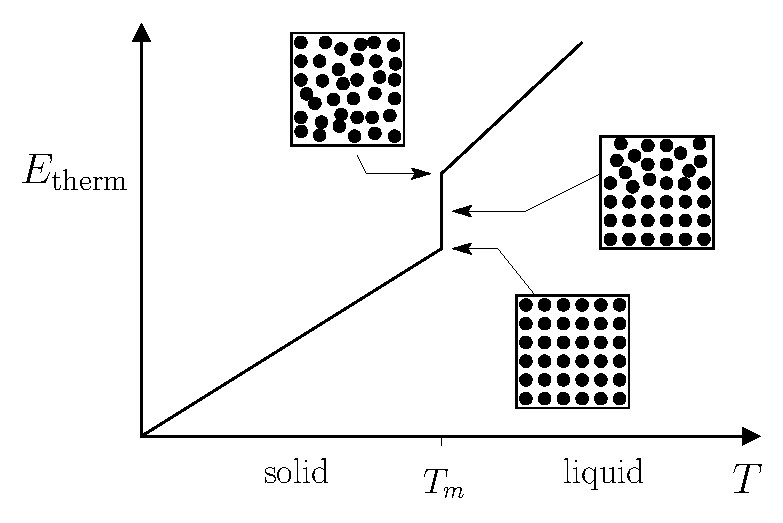
\includegraphics[width=3in]{liquids_and_gases/etherm_vs_t.eps}
\caption{Shown is $E_\text{therm}$ versus $T$ for one mole of a
  typical material.  The slopes in the solid phase and liquid phase
  are the molar specific heats, which are not typically equal to each
  other.  The vertical jump at $T_m$ represents the latent heat of
  fusion, i.e., the amount of thermal energy required to change
  phase.}
\label{fig:etherm_vs_t}
\end{center}
\end{figure}

\begin{example}{Melting lead}
  Calculate the amount of thermal energy that has to be added to 3.0 
  moles of lead at room temperature to melt $\frac{2}{3}$ of the lead. 

  \solution
  This is a two-part process.  First the temperature of the solid lead 
  solid must be raised to its melting temperature.  {\em Then} the 
  lead can be melted.

  In the first part of the process the temperature of all of the lead 
  increases to $600\units{K}$.  The thermal energy change corresponding 
  to this is given by 
  \begin{align}
    \Delta E_\text{therm}^{(1)} & = n_1C\Delta T \nonumber \\ 
    & = 3.0\units{mol}\times 26.6\units{J/mol$\cdot$K} \times
        (600\units{K} - 295\units{K}) \nonumber \\
    & = 24.3 \units{kJ}
  \end{align}
  In the second part of the process the phase changes, so the 
  thermal energy change necessary to melt two moles of the lead is given by
  \begin{align}
    \Delta E_\text{therm}^{(2)} & = n_2 L_f \nonumber \\ 
    & = 2.0\units{mol} \times 4.77\times 10^3\units{J/mol} \nonumber \\
    & = 9.5\units{kJ}
  \end{align}
  Combining these two thermal energy changes gives
  \begin{align}
    \left(\Delta E_\text{therm}\right)_\text{total} 
    & = \Delta E_\text{therm}^{(1)} + \Delta E_\text{therm}^{(2)} \nonumber \\
    & = 24.3\units{kJ} + 9.5\units{kJ} \nonumber \\
    & = 33.8\units{kJ} \
  \end{align} 
  In this calculation, we used the measured value for the molar
  specific heat for lead (see Table \ref{table:material_properties}).
  We could have used the Dulong-Petit (ball-spring) approximation ($C
  = 3R$) which would have given us a result very close to the value
  that we calculated here.

  Note also that if we wanted to start with 2 moles of liquid lead 
  and 1 mole of solid lead both at $600\units{K}$, and cool it down to 
  a solid at room temperature, the same calculation would
  tell us how much thermal energy we would need to {\em remove}.  It
  would also be $33.8\units{kJ}$.
\end{example}


%We can make an estimate for the magnitude of the latent heat.  The
%melting temperature was determined by the energy $k_BT_m$ required to
%stretch the molecular bond by an amount $d/10$.  In the liquid state
%the molecules are not so neatly arranged as in the solid state, so the
%bonds are even farther stretched. The energy required for this
%additional stretching is the latent heat of fusion, which should be an
%energy comparable to $k_BT_m$.  It turns out that
%\begin{equation}
%  L_f \approx N_A k_B T_m = R T_m
%\end{equation}
%is a decent rough estimate for the latent heat of fusion for one mole
%of material.
%
%Interestingly, we can use the same latent heat whether we are adding
%thermal energy to  a solid to melt it, or removing thermal energy from
%a liquid to solidify it.  The latent heat merely reflects the
%potential energy difference of the solid versus liquid configuration
%of molecules.

For most substances, there exists a boiling point separating a liquid
phase from a gas phase.  At the molecular level, the liquid state has
nearly solid-like density, with molecules packed close together and
fairly near the minimum of the potential well.  The transition to the
gas phase requires pulling these molecules apart and setting them
free, where they have no neighbors.  Let $E_\text{bind}$ be the depth
of the potential well, that is, $E_\text{bind}$ is the amount of
energy needed to bring a pair of molecules from their equilibrium
separation to far apart from each other (see
Fig.~\ref{fig:boiling}(a)).  Vaporization (or boiling) occurs roughly
when $k_BT\approx E_\text{bind}$, so we can estimate the boiling
temperature as
\begin{equation}
  T_v\approx\frac{E_\text{bind}}{k_B}.
\label{eq:t_v}
\end{equation}

\begin{example}{Molecular Binding Energy}
  Estimate the molecular pair binding energy $E_\text{bind}$ for
  copper, using the information in
  Table~\ref{table:phase_transitions}.  \solution Copper vaporizes at
  $T_v = 2835\units{K}$, so we may estimate
  \begin{equation}
    E_\text{bind}^{\rm Cu} \approx k_B T_v = (1.38\times 10^{-23}\units{J/K})
    (2835\units{K}) = 3.91\times 10^{-20}\units{J}.
  \end{equation}
  A convenient energy unit for describing molecular bonds is the
  electron volt (eV), defined as
  \begin{equation}
    1\units{eV} = 1.60\times 10^{-19}\units{J}.
  \end{equation}
  In terms of electron volts, then,
  \begin{equation}
    E_\text{bind}^{\rm Cu} = 
    \frac{3.91\times 10^{-20}\units{J}}{1.60\times 10^{-19}\units{J/eV}} 
    = 0.245\units{eV}
  \end{equation}
\end{example}

\begin{figure}
\begin{center}
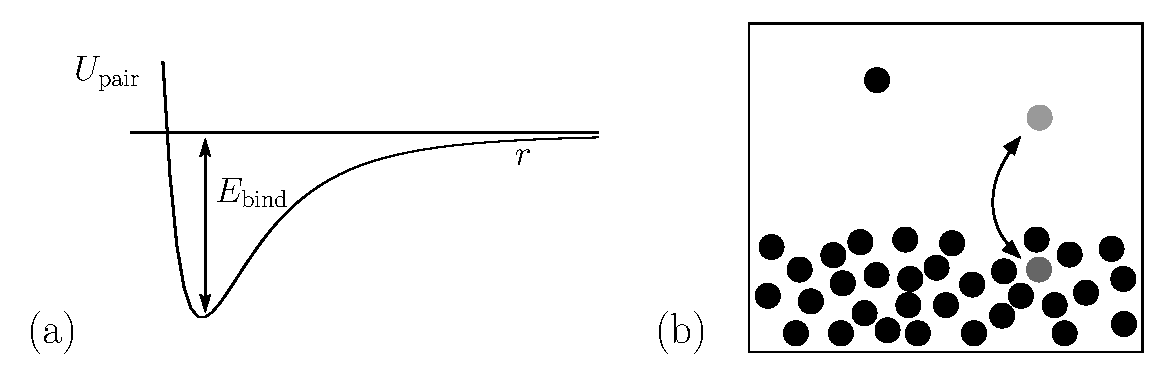
\includegraphics[width=4.4in]{liquids_and_gases/boiling.eps}
\caption{(a) The pair potential depth $E_\text{bind}$.  (b) Removing a particle
from the liquid state requires an energy of about 10--12$E_\text{bind}$.}
\label{fig:boiling} 
\end{center}
\end{figure}

Like with melting, vaporization requires an input of thermal energy.
As thermal energy is added, the temperature remains fixed at the
vaporization temperature, while an increasing amount of liquid gets
converted to gas.  The amount of energy required to convert a mole of
a substance from liquid to gas is called the {\it latent heat of
  vaporization}.  This is used much the same way as the latent heat of
fusion:
\begin{equation}
  |\Delta E_\text{therm}| = nL_v. \qquad\text{(vaporize/condense)}
\end{equation}
As before, $\Delta E_\text{therm}$ is positive if we are adding
thermal energy to vaporize, and it is negative if we are removing
thermal energy to condense.

%We can estimate this energy by realizing that a
%sphere in three dimensions surrounded by spheres of the same size has
%typically 10--12 neighbors.  This is illustrated in
%Fig.~\ref{fig:boiling}(b), though the number of neighbors appears
%smaller because it is a two-dimensional drawing.  Evidently it is
%necessary to add an energy of about $12E_\text{bind}$ to convert a molecule
%from the liquid state to the gas state.\footnote{This estimate takes
%  into account the additional energy required to make space for the
%  new gas molecule.}  We can relate this to the vaporization temperature
%via Eq.~\ref{eq:t_v} and get a ``rule of thumb'' for the latent
%heat of vaporization
%\begin{equation}
%L_v \approx N_A(12E_\text{bind}) \approx 12 N_A k_BT_v  = 12RT_v.
%\end{equation}
%Compared to the latent heat of fusion,
%we see that this latent heat is rather large!  The thermal energy of
%copper from solid to liquid to gas is shown in
%Fig.~\ref{fig:copper_etherm}.  Note that the same latent heat applies
%whether boiling a liquid or condensing a gas: in the former case the
%thermal energy is being added, while in the latter case it is being
%removed.
%
%\begin{figure}
%\begin{center}
%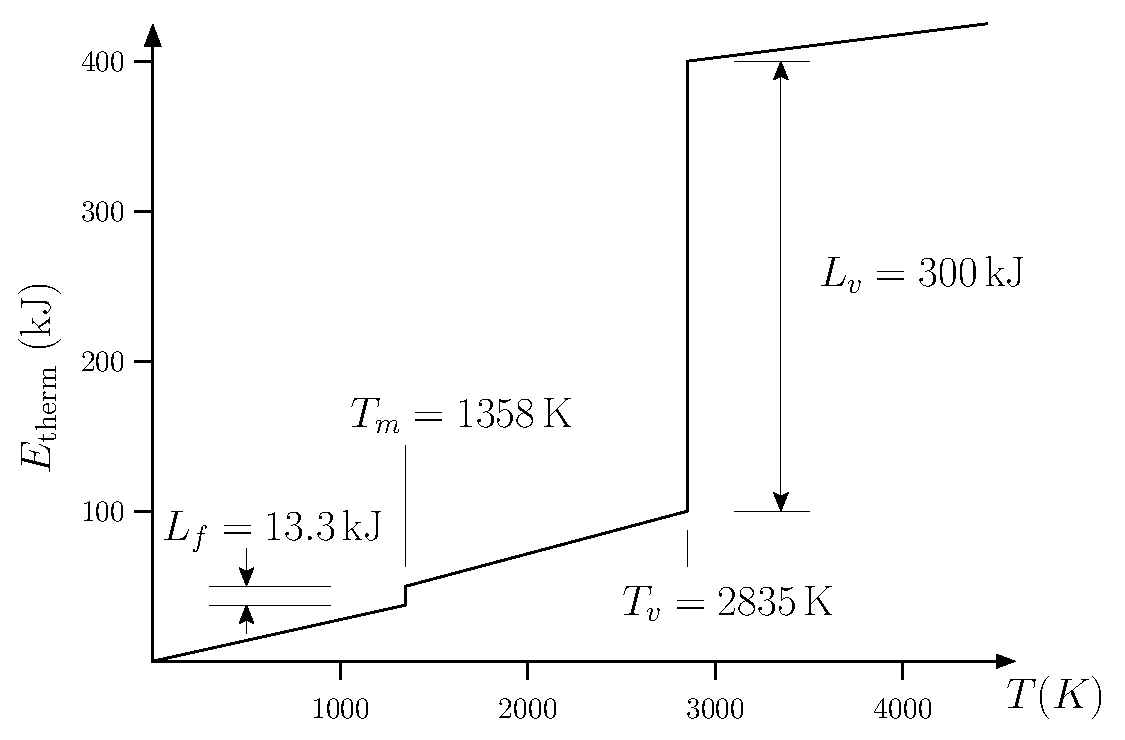
\includegraphics[width=4in]{liquids_and_gases/copper_etherm.eps}
%\caption{$E_\text{therm}$ versus $T$ for one mole of copper as it goes
%  from solid to liquid to gas.  The latent heat of vaporization is
%  large!  Within the phases, the slope indicates the molar specific
%for that phase.}
%\label{fig:copper_etherm}
%\end{center}
%\end{figure}

One final comment about latent heat and phase transitions: the amount
of heat needed to melt or boil most common materials is quite large.
Just looking at Tables \ref{table:material_properties} and
\ref{table:phase_transitions}, you can see that it is necessary to add a
``k'' to the units for latent heats $L_f$ and $L_v$ (versus the units
for molar specific heat $C$) because we are usually talking about
thousands of Joules of energy to cause a phase transition for each
mole of the substance.  This is a very important result with {\it
  lots} of practical applications.  For example, this is the reason
why ice is so good at cooling your drink; it isn't the low {\em
  temperature} of the ice that is important, rather it is the large
amount of energy that the ice absorbs when it melts that does such a
good job of cooling your drink.  Phase transitions are used {\em all
  the time} in cooling and heating applications.  A standard air
conditioner or refrigerator typically uses some substance (e.g.,
freon) whose condensation and vaporization play a key role in the
cooling process.  And your body uses phase transitions to keep cool on
hot summer days.  Sweat (water) on your skin vaporizes, and most of
the energy needed for this phase transition comes from your body.
This is how you can manage not to overheat even if the surrounding air
temperature is greater than your body temperature.  So, we would all
be dead were it not for phase transitions.

\section{Pressure}

Liquids and gases push outwardly on their surroundings.  To describe
this push we introduce the concept of {\it pressure}.  Consider a
liquid or a gas enclosed in some container, and focus on one wall of
the container with area $A$, such as shown in
Fig.~\ref{fig:gas_pressure}.  The fluid pushes on the wall in the
perpendicular direction with a force of magnitude $F$.  Pressure is
then the force per area
\begin{equation}
  p=\frac{F}{A},
\end{equation}
and has units N/m$^2$.  This combination of units is given the name
pascal (Pa), that is, $1\units{Pa} = 1\units{N/m$^2$}$.  Atmospheric
pressure is given by
\begin{equation}
  p_\text{atm} = 1.01\times 10^{5} \units{Pa} = 101\units{kPa}.
\end{equation}
Note that pressure applies to more than just liquids and gases.  Any
time that there is a force exerted on a surface, you can define a
pressure simply by dividing that force by the surface area.
Conceptually, the pressure indicates how ``spread out'' the force is,
i.e., if the same force is exerted over a larger surface area, then
there is less force per unit area (smaller pressure) and each part of
the surface experiences a smaller force.  That is why, for example, it
is useful to wear snowshoes with a large surface area when walking
over fresh snow --- the downward force you exert on the ground is
spread over a larger area, resulting in a smaller pressure on the
snow, so the snow doesn't collapse.

Pressure does not have a direction.  If we consider some point in the
fluid, pressure is an outward push in all directions.  This outward
push is balanced by an identical outward push from a neighboring
region of the gas.  Only at the boundaries of the gas is there an
imbalance --- here the enclosed gas is only pushing from inside --- and
that is where we can measure the pressure.  And note:  {\bf a gas
can ONLY push on a surface; it NEVER pulls!!!}

\begin{figure}
\begin{center}
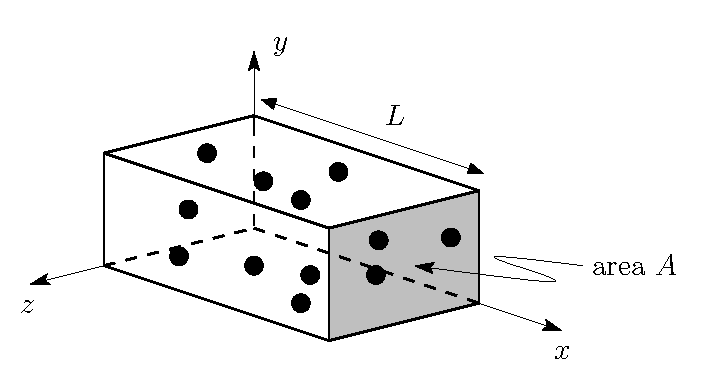
\includegraphics[width=3.5in]{liquids_and_gases/gas_pressure.eps}
\caption{A gas enclosed in a container of length $L$, with the shaded
wall having area $A$.}
\label{fig:gas_pressure}
\end{center}
\end{figure}

We can use our picture of the gas state to derive the pressure of a
gas.  In the {\it ideal gas} approximation we ignore collisions
between the molecules entirely, and treat each molecule as bouncing
back and forth between the walls of the container.  The particles bouncing
off the walls exert a force on the wall, and this is precisely the 
origin of pressure.

\newpage

\begin{example}{Pressure and Balloons}
  Explain qualitatively how the gas inside an inflated balloon
  prevents the balloon from collapsing.

  \solution When a balloon is inflated, the rubber is stretched in all
  directions, resulting in an increased tension.  At every point along
  the surface of the balloon fabric, the tension pulls in all
  directions along the surface.  Because of the curvature of the
  balloon, these tension forces add up to give a net inward tension
  force.

  The inward components of the tension do not cause the balloon to
  collapse because there is an outward force due to air molecules
  trapped within the balloon bouncing off the inner surface of the
  balloon.  Each time a molecule bounces off a piece of the balloon,
  it gives that piece a small outward kick.  Of course, there are also
  molecules outside the balloon, and each time one of these bounces
  off the balloon, it gives a small inward kick.  If the outward and
  inward forces were balanced, which is what happens with an open
  balloon, then the net force would be the tension force, and the
  balloon would rapidly shrink.

  But what if the collisions from the inside molecules are more
  frequent and/or harder collisions?  Consider that there are
  around $10^{23}$ gas molecules in a typical balloon, and they are
  moving quite fast at typical room temperatures (see Example
  \ref{example:vtherm}).  There are a {\bf lot} of collisions occurring
  each second between gas molecules and the inside of the balloon.
  The result of all of these collisions is an outward force exerted on
  the balloon fabric by the gas molecules.  This outward gas force
  opposes the inward components of the tension {\it and} the inward
  force due to the collisions of all the gas molecules on the outside,
  and as a result the balloon does not collapse.
\end{example}

\section{The Ideal Gas Law}

Now that we know how it is that a gas can exert a pressure, we
can use these ideas --- along with the previous discussion of
thermal velocities of gas molecules --- to calculate how the
pressure relates to the temperature of the gas, the number of gas
molecules (or moles) and the geometry of the container holding the
gas.  From this we will derive one of the most useful 
relations in thermodynamics: the {\em ideal gas law}.

 A collision with a wall is shown in Fig.~\ref{fig:collide_wall}.
 Note that the $x$-component of velocity changed sign, while the
 $y$-component of the velocity was unchanged.  If we focus on $v_x$,
 we can see that the molecules in Fig.~\ref{fig:gas_pressure} will
 bounce off the shaded wall and change the sign of $v_x$, then a time
 $L/v_x$ later they will bounce off the back wall and head back toward
 the shaded wall.  They will likely bounce off the side walls en
 route, but this has no effect on $v_x$, so we can ignore it.  Thus
 the time between collisions on the shaded wall is $\Delta t = 2L/v_x$
 (the factor of two coming from the trip away and then back).


The force on the wall due to the particle is zero in between
collisions, and then very abruptly some non-zero value during the
collision.  Viewed as a function of time, the force would be a series
of spikes, since each collision is short in duration, and then there
is no force while the particle travels to the other side of the
container and back again. What we feel as steady pressure is the time
average of many collisions, so we would like to obtain an average of
this force over time.  


\begin{figure}
\begin{center}
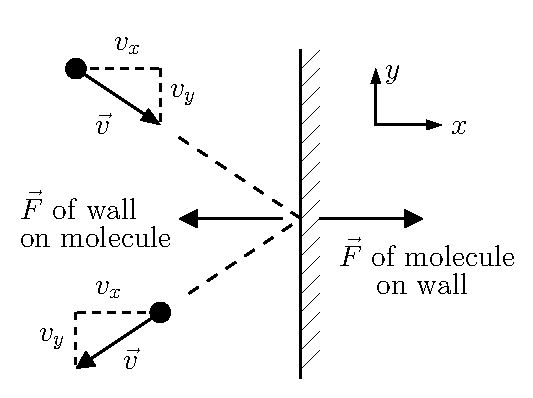
\includegraphics[width=2.6in]{liquids_and_gases/collide_wall.eps}
\caption{The $x$-component of velocity changes sign, while the $y$-component
of velocity is unchanged.}
\label{fig:collide_wall}
\end{center}
\end{figure}

We can calculate this time averaged force first by noting that the force
of the molecule on the wall is, by Newton's third law, equal and opposite
the force of the wall on the molecule.  The force of the wall on the molecule
causes a change in the $x$-component of momentum, $p_x$ (see 
Fig.~\ref{fig:collide_wall}).  Note that the symbol $p$ here, and in the 
next two equations,  refers to momentum, not pressure. We apologize for 
the fact that the standard symbols for these quantities are the same
(but there are only so many letters to use).  The momentum change is 
given by 
\begin{equation}
\Delta  p_x  = - mv_x - m v_x = -2mv_x.
\end{equation}
This momentum change happens once every time interval of $\Delta t =
2L/v_x$ (the travel time between collisions), so we can conclude the
average force of the wall on the molecule is
\begin{equation}
F_{{\rm avg},x} = m a_\text{avg}= \frac{m \Delta v_x}{\Delta t} =\frac{\Delta p_x}{\Delta t} = -\frac{2mv_x}{2L/v_x} =
-\frac{mv_x^2}{L}.
\end{equation}
The average force of the {\it molecule on the wall} is then
equal and opposite.  If we consider all $N$ molecules, then we can
conclude
\begin{equation}
F_{\text{on wall},x} = \sum_i \frac{m v_{i,x}^2}{L}
\end{equation}
where $v_{i,x}$ is the $x$-component of the velocity $\vec v_i$ of the
$i$th particle.
We can appeal to the equipartition theorem, which tells us
\begin{equation}
\Bigl\langle\sum_i {\textstyle\frac{1}{2}} m v_x^2\Bigr\rangle = N
\bigl({\textstyle\frac{1}{2}}k_BT\bigr),
\end{equation}
and so the average force on the wall is given by
\begin{equation}
F_{\text{on wall},x} = \frac{Nk_BT}{L}.
\end{equation}
Finally, we use the definition of pressure to conclude
\begin{equation}
p = \frac{F_{\text{on wall},x}}{A} = \frac{Nk_BT}{AL} = \frac{Nk_BT}{V}
\end{equation}
where we have used $V=AL$ (see Fig.~\ref{fig:gas_pressure}).  This
last relation holds regardless of the shape of the container, and we
have thus derived the {\it ideal gas law}
\begin{equation}
pV = N k_BT \qquad \text{or}\qquad pV = nRT.
\label{eq:ideal_gas_law}
\end{equation}
This is another universal law where the details of the molecules are
irrelevant: the molecular mass canceled out, and any interaction
forces between the molecules negligible as long as the gas is dilute
enough.

This is an extremely accurate law for most gases at room temperature and
higher temperatures.  Note also that it does not depend on the mass of
the gas molecule, or whether it is diatomic or monatomic.

In Eq.~(\ref{eq:ideal_gas_law}), both sides of the equations have units
of energy.  If we use SI units, pressure should be measured in pascal,
and volume should be measured in cubic meters.   However, we may take
advantage of the relation
\begin{equation}
1\units{J} = (1\units{Pa})(1\units{m$^3$}) = 
(10^{-3}\units{kPa})(10^3\units{L}) = (1\units{kPa})(1\units{L}),
\end{equation}
where $L$ is liters.  This tells us we can use kilopascals and liters and
the product $pV$ will turn out to be joules.  

\begin{example}{Volume of a Mole of Gas}
  Calculate the volume in liters occupied by a mole of ideal gas at a
  temperature of $22^\circ\units{C}$ and atmospheric pressure.

  \solution Starting from Eq.~(\ref{eq:ideal_gas_law}), we solve for
  $V$:
  \begin{equation}
    V = \frac{nRT}{p} = \frac{(1\units{mol})(8.31\units{J/mol$\cdot$K})
      (295\units{K})}{101\units{kPa}} = 24.2\units{L}.
  \end{equation} 
  Note that we had to convert temperature from Celsius to Kelvin in
  this calculation.  {\bf This is important:} you {\bf always} have to
  use Kelvin for the temperature when using the ideal gas law.
\end{example}

\begin{exampleb}{Using Ratios in the Ideal Gas Law}
  An ideal gas at a temperature $50^{\circ}$ C is in a car piston.
  The piston compresses the gas to 1/3 of its original volume.  The
  pressure increases by a factor of 5 during this process.  Calculate
  the new temperature of the gas in the piston.

  \solution We don't know the volume, pressure or number of moles of
  gas at any point in this problem, so we will have to solve this
  problem using ratios.

  First, we need to convert temperature to Kelvin: $T = (50+273)
  \units{K} = 323 \units{K}$.  Next, write down the ideal gas law: $pV
  = nRT$.  We are interested ultimately in the final temperature, so
  re-write this as:
  \begin{equation}
    T = \frac{pV}{nR}
  \end{equation}
  This holds both initially and after the compression, so $T_1 =
  p_1V_1/(n_1R)$ and $T_2 = p_2V_2/(n_2R)$.  
\begin{equation}
  \frac{T_2}{T_1} = \frac{\displaystyle\left(\frac{p_2V_2}{n_2R}\right) }
 {\displaystyle\left( \frac{p_1V_1}{n_1R}\right) } 
  = \frac{p_2}{p_1}\frac{V_2}{V_1},
\end{equation}
since $n_2 = n_1$ and $R$ is a constant.  So, the final temperature is
\begin{equation}
  T_2 = T_1 \cdot \frac{p_2}{p_1}\cdot\frac{V_2}{V_1} = 
  (323\units{K})\cdot 5 \cdot \frac{1}{3}
  = 538 \units{K} ,
\end{equation}
or $(538 - 273)^{\circ}\units{C} = 265^{\circ}\units{C}$.

Note that when using ratios to determine a new value for the pressure
or volume, it doesn't matter what units we use for those quantities
because the units will cancel between numerator and denominator. 
%For example, if the initial volume is in cm$^3$, then the final volume
%will be in cm$^3$.
Though it is still always necessary to use Kelvin for temperature.
\end{exampleb}

\newpage

\section*{Problems}
\markright{PROBLEMS}

%[Assigned: A46 - sucking tubes. A47 - dunking birds.]

\begin{problem} {\bf Melting iron}
  \begin{enumerate}
  \item Use your results from
    Problem~\ref{chapter:thermal_energy}.\ref{problem:ball-spring_iron}
    to estimate the typical thermal displacement for atoms in a chunk
    of solid iron at room temperature.  (Assume a room temperature of
    $22^{\circ}\units{C}$.)  Compare your result to the typical
    lattice separation for the iron atoms.  Based on this result and
    the Lindemann criterion, explain why it is reasonable that iron is
    a solid at room temperature.

  \item Now, assuming that iron melts when the typical displacement is
    one-tenth the lattice separation (i.e., $x_\text{therm} \approx
    d/10$, which is the Lindemann criterion), estimate the melting
    temperature of iron.  Compare your result to the experimental
    value.

  \item Write a sentence explaining in your own words why the melting
    temperature should be related to the typical thermal displacement
    $x_\text{therm}$.  Don't worry so much about the factor $1/10$ in
    the Lindemann melting criterion, but your explanation {\bf should}
    state why melting occurs when $x_\text{therm}$ gets sufficiently large.
  \end{enumerate}
\label{problem:iron_melting}
\end{problem}

%\begin{problem}  % maybe replace with something more useful!
%  Of the substances listed in Table~\ref{table:phase_transitions}, one
%  deviates significantly (more than a factor of two) from the estimate
%  that the latent heat of fusion is roughly $k_BT_m$ per molecule.
%  Identify the substance.  Can you make a guess why?
%\label{problem:sesame_street}
%\end{problem}

\begin{problem}
Calculate the thermal speed at temperature $22^\circ\units{C}$ of
\begin{enumerate}
\item molecular oxygen (O$_2$)
\item methane (CH$_4$)
\item carbon dioxide (CO$_2$)
\end{enumerate}
\label{problem:thermal_speeds}
\end{problem}

\begin{problem}
A 100\units{g} piece of ice at $0^\circ\units{C}$ is placed into a
container holding 200\units{g} of water, initially at temperature
$25^\circ\units{C}$.  Heat flows from the water to the ice, cooling the water
and melting the ice. 
% The specific heat of water is
%$C=75.3\units{J/mol$\cdot$K}$.
\begin{enumerate}
\item Calculate how many moles of ice and how many moles of water are
initially present.
\item  Determine how much 
heat flows out of the water in cooling to  $0^\circ\units{C}$.
\item Determine how many moles of ice are melted by this added heat.
\end{enumerate}
\label{problem:water_calorimetry}
\end{problem}

\begin{problem}
Compare two containers of the same ideal gas; each container has 
the same volume and the same number of molecules.  The temperature 
of the gas in the first container is twice the temperature in the 
second container,
$T_1=2T_2$.  Find the following ratios
\begin{enumerate}
\item $v_\text{therm,1}/v_\text{therm,2}$.
\item $K_\text{molec,1}/K_\text{molec,2}$.
\item $p_1/p_2$.
\end{enumerate}
\label{problem:ideal_gas_ratios}
\end{problem}

\begin{problem}
How many moles are in 3 liters of ideal gas at pressure $200\units{kPa}$
and temperature $100^\circ\units{C}$?
\label{problem:ideal_gas_moles}
\end{problem}

\begin{problem} 
  Using the vaporization temperature of water to estimate the pair
  binding energy for water molecules.
%\begin{enumerate} 
%\item Calculate the ratio $L_v/k_BT_v$ for each substance in
%  Table~\ref{table:phase_transitions}.  Compare your results with the
%  ``rule of thumb'' presented in section~\ref{section:boiling}.
%\item Estimate the pair binding energy for water molecules.
%\end{enumerate}
\label{problem:heat_of_vaporization}
\end{problem}


\begin{problem}
Calculate the speed of sound in a gas of pure molecular hydrogen at a
temperature of $22^\circ\units{C}$.
\label{problem:speed_of_sound}
\end{problem}


% handins begin

%[Handins begin here.  A48 - blow dart suction]


\begin{problem}
One mole of water at $20^\circ\units{C}$ has 20\units{kJ} of thermal
energy added.  Calculate the number of moles which remain in the liquid
state.
\end{problem}


\begin{problem}
Rank the following according to the speed of the molecules at room
temperature, from fastest to slowest:
\begin{enumerate}
\item copper (solid)
\item water (liquid)
\item krypton (gas)
\item molecular nitrogen (gas)
\end{enumerate}
\end{problem}


\begin{problem}
A fixed amount of ideal gas is at temperature $25^\circ\units{C}$,
volume $4.0\units{L}$ and pressure $100\units{kPa}$.  The temperature
of the gas is increased to $80^\circ\units{C}$ while the volume is
decreased to $3.2\units{L}$.  Determine the new pressure.
\end{problem}

\begin{problem}
  For silver, the ball-spring parameters are $m=1.79\times
  10^{-25}\units{kg}$, $d=2.58\times 10^{-10}\units{m}$, and
  $k_{sp}=21.4\units{N/m}$.  Based on this information, estimate the
  melting temperature and latent heat of fusion for silver.  
\end{problem}

% Problems using Schroeder's molecular dynamics applet - very rough drafts

%\begin{problem}
%{\bf Solid-liquid coexistence.}  For this problem you will use the
%molecular simulation applet available online.  
%(A link to the simulations
%can be found on today's Calendar page for today's lecture.)
%Load in the preset [preset will specify the number of particles, 
%a little bit of gravity, and a thermal energy that results 
%in a busy liquid phase].  Vary the thermal energy until you 
%find a value gives you
%liquid-solid coexistence.  Determine the thermal energy values
%corresponding to
%\begin{enumerate}
%\item when the system has just left the liquid-solid coexistence and
%  completely solidified.
%\item when the system has just left the liquid-solid coexistence and
%  completely melted.
%\item How would expect the molecular kinetic energies to compare at
%  these two points?  [they woudl be essentially equal, since the
%    temperature hasn't been changing, only the phase]
%\end{enumerate}
%\end{problem}

%  500 atoms, atom size=10, gravity=0.1, timestep =0.004, animation speed=50
% works well for a liquid.

%\begin{problem}
%{\bf Diatomic versus monatomic gases.} For this problem you will use
%the molecular simulation applet available online. 
%(A link to the simulations can be found on today's 
%Calendar page for today's lecture.) In
%fact, you will need to open two browsers and start up two separate
%simulations.  In the first simulation, load the monatomic ideal
%gas preset.  In the second simulation, load the diatomic gas preset.
%You also might want to reduce the animation speed so that the motion
%is easy to follow (on faster computers, an animation speed of 10 is
%sometimes good).
%\begin{enumerate}
%\item Assign the same value of thermal energy to each system.  (You
%  might want to click ``Slower'' a few times to get to manageable
%  speeds.  For reference, a thermal energy of around 80 works well).  Note
%  that they have the same number of particles, so the average energy
%  per particle should be equal in the two cases.  How does it look?
%  Are they moving at comparable speeds?
%\item No, they aren't.  Now increase the thermal energy of the system
%  that looks to be moving slower until, roughly by eye the molecules
%  in the two systems appear to be moving at comparable speeds.  Record
%  your $E_\text{therm}$ values for the diatomic and monatomic gases.
%\item What's going on here?  (Hint:  for a monatomic gas, the energy
%  all goes into translation of the atoms.  For a diatomic molecule,
%  where does the energy go to?)  Can you explain your answer to (a)?  Your
%  explanation should lead to a prediction for the ratio of the
%  $E_\text{therm}$ values.  What is the prediction, and how do your
%  values compare?  
%\end{enumerate}
%\end{problem}

\begin{problem} {\bf Let's play microwave.}  This is just fun, and
  you've got to do it.  Load up the molecular dynamics applet, select
  the solid preset, and click ``Start''.  Now we're going to melt the
  solid without adding heat.  This is exactly what a microwave oven
  does: the microwaves do work, pushing and pulling molecules around,
  and this gets converted to thermal energy.  So let's do the same
  thing.  You can ``pull'' a molecule by clicking on it and dragging
  it.  Reach in and pull on a molecule, and then wait and watch how the
  system responds.  Now do it again.  Keep doing it until you've fully
  melted the solid.  (Notes: it might help to reduce the ``Animation
  speed'' so that you can see what is going on.  You also might have
  to pull your mouse a large distance quickly before letting go when
  ``pulling'' a molecule.)

\begin{enumerate}
\item Describe what you observe in the simulation and what you had to
  do to melt the solid by pulling on individual atoms.  {\bf
    Question:} Why would pulling on just one or two individual atoms
  melt the entire solid?

\item Now think of something else cool to do with the applet.  Write a
  few sentences describing what you did and what you found.
\end{enumerate}
\end{problem}

\begin{problem}
  Aquaman buys a balloon filled with a fixed amount of helium from a
  street vendor in New York City on a hot $37^{\circ}\units{C}$ day.
  He measures the pressure inside the balloon to be $1.1\units{atm}$
  ($1\units{atm}=101\units{kPa}$).  When he arrives at the underwater
  city of Atlantis, he discovers that the balloon is now 0.40 times
  the original volume.  His thermometer indicates that the ocean has a
  temperature of $2^{\circ}\units{C}$.  Determine the pressure inside
  the balloon.
\label{problem:aquaman}
\end{problem}

\begin{problem}
  Let's consider the ideal gas law $pV = nRT$ qualitatively from a
  perspective of molecules of the gas hitting the shaded side of a
  container, as shown in Fig.~\ref{fig:ideal_gas_problem}.
  \begin{figure}[ht]
    \begin{center}
      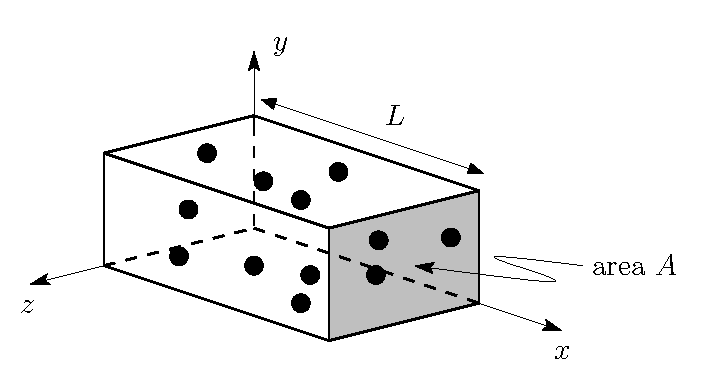
\includegraphics[width=3.5in]{liquids_and_gases/gas_pressure.eps}
      \caption{For problem~\ref{problem:ideal_gas_law}.  Gas in a
        container of length $L$ and cross section $A$.}
      \label{fig:ideal_gas_problem}
    \end{center}
  \end{figure}
  \begin{enumerate}
  \item Considering collisions of gas molecules with the wall, explain
    qualitatively why the pressure of a gas increases if the
    temperature of the gas increases, with everything else constant.
    There are two different reasons why increasing the temperature
    increases the pressure.
  \item Explain qualitatively why the pressure of a gas increases if
    the number of moles of gas molecules in the gas increases, with
    everything else constant.
  \item Explain qualitatively why the pressure increases if the volume
    of the container holding the gas decreases, with everything else
    constant.  There are actually two different reasons why decreasing
    the volume increases the pressure: one is a result of decreasing
    $L$ and the other is a result of decreasing $A$.
  \end{enumerate}
  \label{problem:ideal_gas_law}
\end{problem}
\newpage

\begin{problem}
  In this problem you will make some simplifying assumptions and estimate 
  the pressure of a gas of nitrogen molecules from a microscopic picture 
  of the gas.  Assume that the gas is in a $10\units{cm} \times 
  10\units{cm}\times 10\units{cm}$ box at room temperature, 
  $T = 22^\circ\units{C}$.  The assumptions are:
  \begin{itemize}
  \item All the molecules travel at the speed $v_\text{therm}$ derived 
  in Example~\ref{example:vtherm}.  This is 
  not actually true --- there is a spread in 
  molecular speeds around the average ---
  but $v_\text{therm}$ is a typical speed.
  \item One third of the molecules in the gas travel in the $\pm x$-direction,
  one third travel in the $\pm y$-direction, and one third travel in the 
  $\pm z$-direction.  This is obviously not true, but this assumption will
  simplify the calculations.
  \end{itemize}
 
  \begin{figure}[ht]
    \begin{center}
      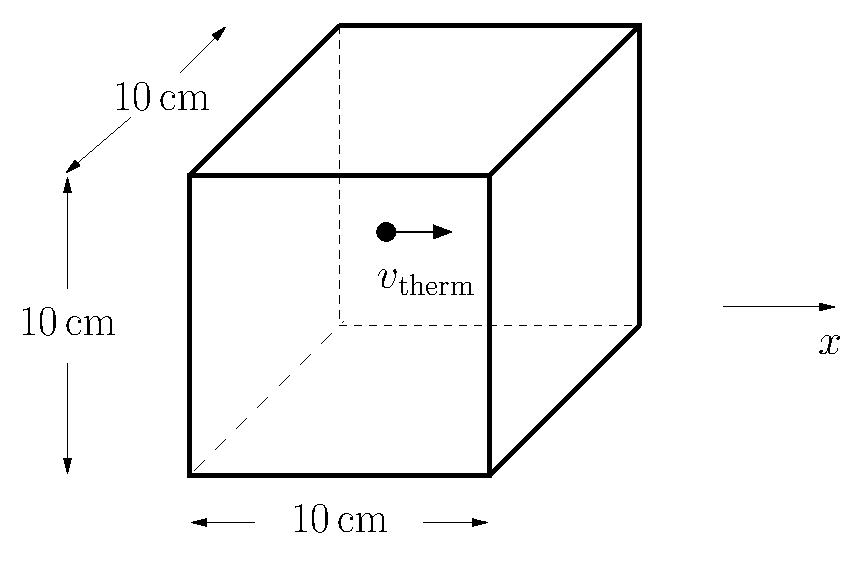
\includegraphics[width=2.5in]{liquids_and_gases/ideal_gas_prob.eps}
      \caption{Figure for problem~\ref{problem:ideal_gas_quant}.}  
      \label{fig:ideal_gas_quant}
    \end{center}
  \end{figure}
  
  \begin{enumerate}
  \item Calculate the numerical value of the {\em change} in the momentum of 
  a single nitrogen molecule traveling in the $x$-direction after it 
  collides elastically with the right wall of the container.  (If you 
  need help determining the speed of the nitrogen molecules, see Example
  \ref{example:vtherm}.)
  \item Calculate the number of times this single nitrogen molecule 
  collides with the right wall of the container in 1 second.
  \item Calculate the total change in momentum of the molecule in 1 second
  due to collisions with the right wall of the container.
  \item Calculate the average force on the right wall of the container 
  due to collisions with the single molecule.
  \item At room temperature and atmospheric pressure, the number density, 
  (i.e., the number of molecules per unit volume) of 
  nitrogen molecules is $2.49\times 10^{19}\units{molecules/cm$^{3}$}$.  
  Use the second of our simplifying assumptions and calculate the 
  average force on the right wall of the container due to all of the 
  molecules in the gas. 
  \item Calculate the pressure that the gas exerts on the right wall
  of the container.  Compare your answer to atmospheric pressure 
  ($1\units{atm} = 1.01\times 10^5\units{Pa}$). 
  \end{enumerate}
  \label{problem:ideal_gas_quant}
\end{problem}
